Foram definidos cinco cenários distintos de teste para avaliar o desempenho do sistema fuzzy Mamdani, conforme apresentado na Tabela~\ref{tab:cenarios}. Cada cenário representa uma combinação específica de temperatura, umidade e número de pessoas, abrangendo situações típicas de ambientes fechados, desde condições amenas até ambientes quentes, úmidos e cheios.

A análise desses cenários permitiu verificar como o sistema fuzzy responde a diferentes condições ambientais, avaliando a recomendação de ventilação para cada caso. Os resultados obtidos para cada cenário foram posteriormente discutidos, considerando tanto os valores quantitativos das técnicas de defuzzificação quanto a interpretação qualitativa das recomendações do sistema.

\begin{table*}[ht]
\centering
\caption{Cenários de teste utilizados nas simulações do sistema fuzzy Mamdani.}
\label{tab:cenarios}
\begin{tabular}{c|c|c|c}
\hline
\textbf{Cenário} & \textbf{Temperatura (°C)} & \textbf{Umidade (\%)} & \textbf{Pessoas} \\
\hline
1 & 28 & 80 & 15 \\
2 & 22 & 50 & 5  \\
3 & 18 & 30 & 2  \\
4 & 32 & 60 & 10 \\
5 & 25 & 90 & 8  \\
\hline
\end{tabular}
\end{table*}


Para compreender o comportamento global do sistema fuzzy Mamdani, foram geradas superfícies fuzzy para cada um dos cinco cenários simulados. Cada cenário representa uma combinação distinta de temperatura, umidade e número de pessoas, permitindo visualizar como a recomendação de ventilação varia conforme as condições do ambiente.
Para cada cenário, foram plotadas três superfícies fuzzy, permitindo analisar a recomendação de ventilação em função das variáveis de entrada. As superfícies correspondem a: (i) ventilação em função de temperatura e umidade (com número de pessoas fixo), (ii) ventilação em função de temperatura e número de pessoas (com umidade fixa) e (iii) ventilação em função de umidade e número de pessoas (com temperatura fixa).

A seguir, apresentam-se e discutem-se os resultados para cada cenário, com referência direta às superfícies correspondentes:

\subsubsection{Cenário 1: Ambiente quente, úmido e cheio}

As Figuras~\ref{fig:superficie-c1-t-u}, \ref{fig:superficie-c1-t-p} e \ref{fig:superficie-c1-u-p} ilustram, respectivamente, a ventilação recomendada em função de temperatura e umidade (pessoas fixas), temperatura e pessoas (umidade fixa) e umidade e pessoas (temperatura fixa) para o Cenário 1.

\begin{figure}[ht]
    \centering
    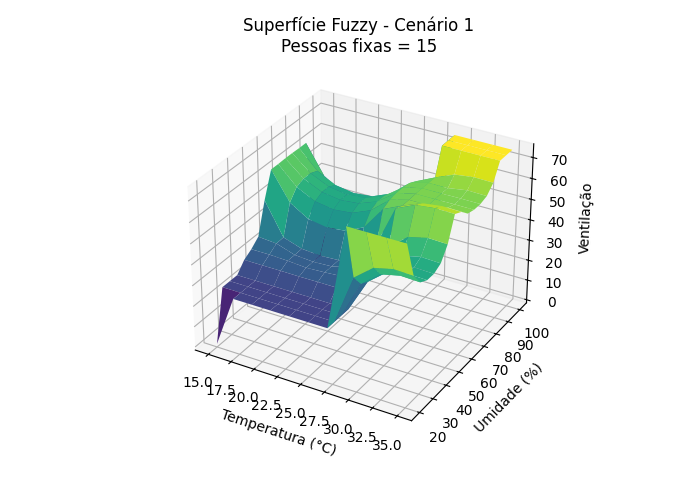
\includegraphics[width=0.48\textwidth]{../img/superficie_cenario1_fixapessoas.png}
    \caption{Ventilação em função de temperatura e umidade, pessoas fixas (Cenário 1).}
    \label{fig:superficie-c1-t-u}
\end{figure}
\begin{figure}[ht]
    \centering
    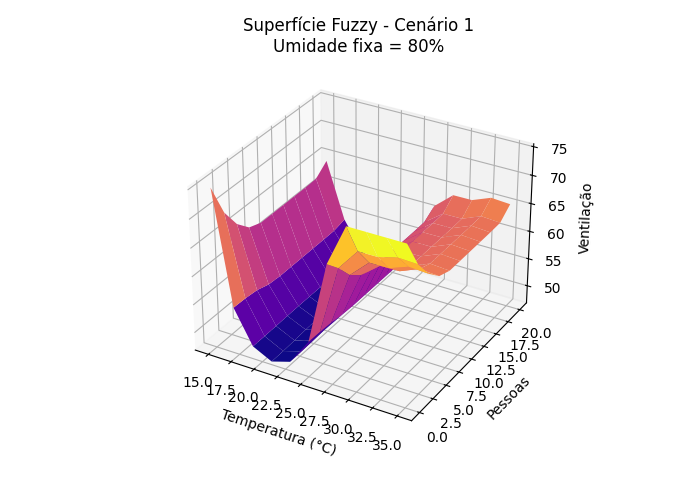
\includegraphics[width=0.48\textwidth]{../img/superficie_cenario1_fixaumidade.png}
    \caption{Ventilação em função de temperatura e pessoas, umidade fixa (Cenário 1).}
    \label{fig:superficie-c1-t-p}
\end{figure}
\begin{figure}[ht]
    \centering
    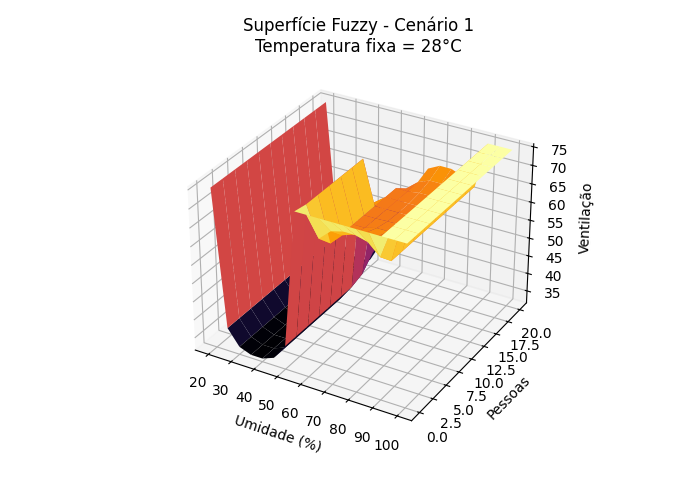
\includegraphics[width=0.48\textwidth]{../img/superficie_cenario1_fixatemperatura.png}
    \caption{Ventilação em função de umidade e pessoas, temperatura fixa (Cenário 1).}
    \label{fig:superficie-c1-u-p}
\end{figure}

No Cenário 1, observa-se que a ventilação recomendada é elevada para altas temperaturas, alta umidade e grande número de pessoas, refletindo a necessidade de maior renovação do ar para garantir conforto térmico.

\subsubsection{Cenário 2: Ambiente ameno e pouco ocupado}

As Figuras~\ref{fig:superficie-c2-t-u}, \ref{fig:superficie-c2-t-p} e \ref{fig:superficie-c2-u-p} apresentam as superfícies fuzzy para o Cenário 2.

\begin{figure}[ht]
    \centering
    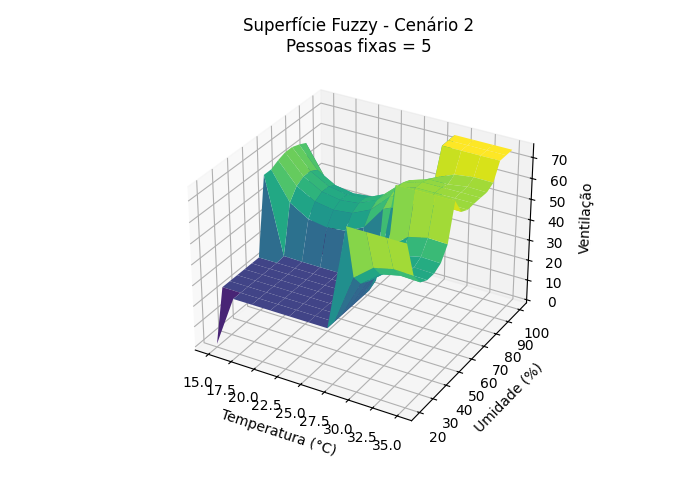
\includegraphics[width=0.48\textwidth]{../img/superficie_cenario2_fixapessoas.png}
    \caption{Ventilação em função de temperatura e umidade, pessoas fixas (Cenário 2).}
    \label{fig:superficie-c2-t-u}
\end{figure}
\begin{figure}[ht]
    \centering
    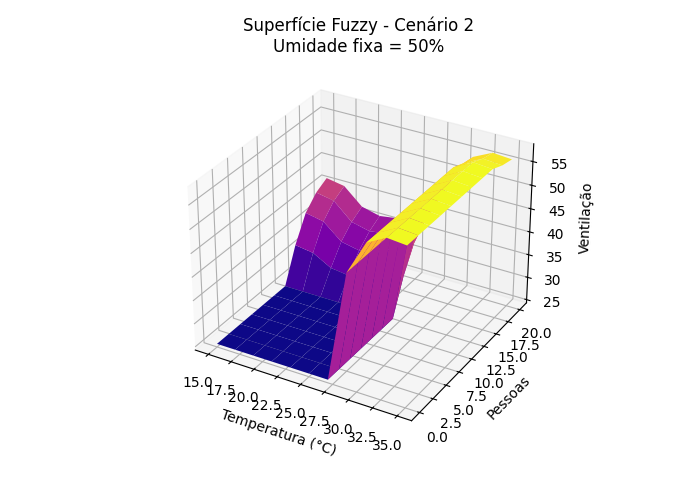
\includegraphics[width=0.48\textwidth]{../img/superficie_cenario2_fixaumidade.png}
    \caption{Ventilação em função de temperatura e pessoas, umidade fixa (Cenário 2).}
    \label{fig:superficie-c2-t-p}
\end{figure}
\begin{figure}[ht]
    \centering
    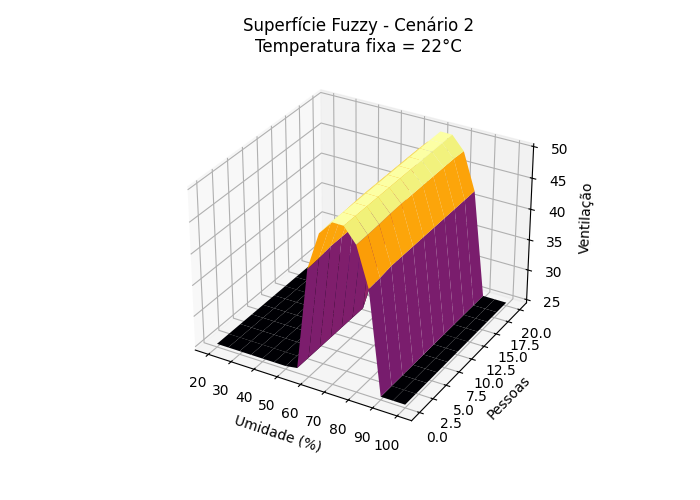
\includegraphics[width=0.48\textwidth]{../img/superficie_cenario2_fixatemperatura.png}
    \caption{Ventilação em função de umidade e pessoas, temperatura fixa (Cenário 2).}
    \label{fig:superficie-c2-u-p}
\end{figure}

Neste cenário, as superfícies mostram que a ventilação recomendada é geralmente baixa, aumentando apenas em situações de temperatura ou umidade elevadas, ou com aumento do número de pessoas.

\subsubsection{Cenário 3: Ambiente frio, seco e vazio}

As Figuras~\ref{fig:superficie-c3-t-u}, \ref{fig:superficie-c3-t-p} e \ref{fig:superficie-c3-u-p} apresentam as superfícies fuzzy para o Cenário 3.

\begin{figure}[ht]
    \centering
    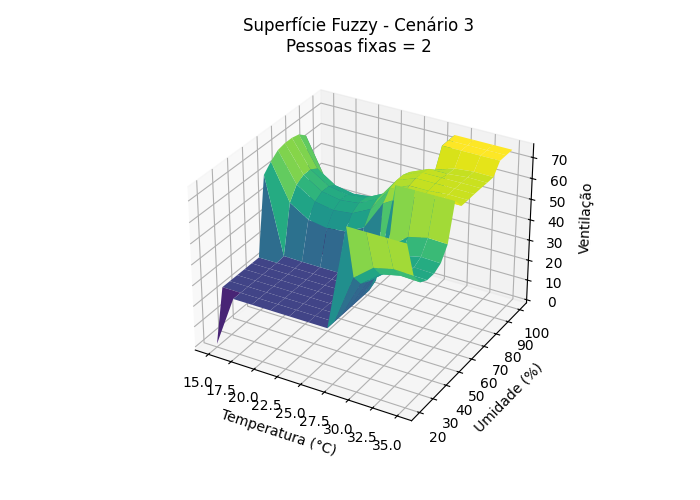
\includegraphics[width=0.48\textwidth]{../img/superficie_cenario3_fixapessoas.png}
    \caption{Ventilação em função de temperatura e umidade, pessoas fixas (Cenário 3).}
    \label{fig:superficie-c3-t-u}
\end{figure}
\begin{figure}[ht]
    \centering
    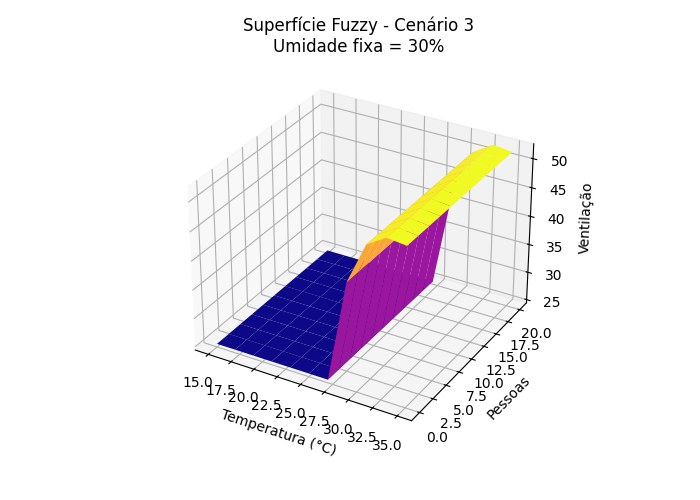
\includegraphics[width=0.48\textwidth]{../img/superficie_cenario3_fixaumidade.png}
    \caption{Ventilação em função de temperatura e pessoas, umidade fixa (Cenário 3).}
    \label{fig:superficie-c3-t-p}
\end{figure}
\begin{figure}[ht]
    \centering
    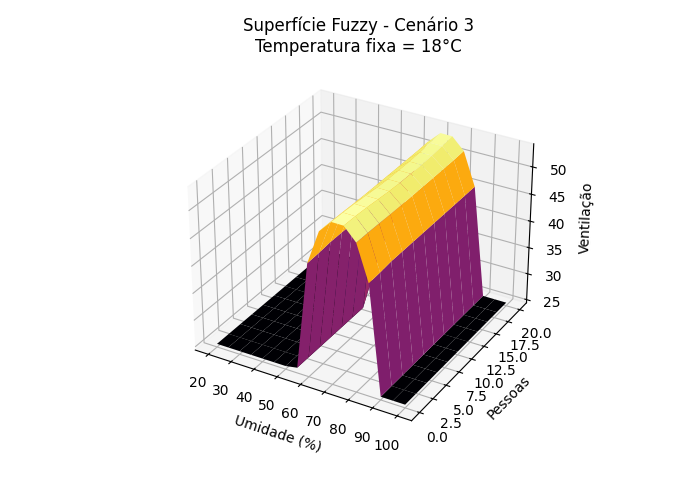
\includegraphics[width=0.48\textwidth]{../img/superficie_cenario3_fixatemperatura.png}
    \caption{Ventilação em função de umidade e pessoas, temperatura fixa (Cenário 3).}
    \label{fig:superficie-c3-u-p}
\end{figure}

No Cenário 3, a ventilação recomendada é predominantemente fraca, pois as condições do ambiente não exigem renovação intensa do ar.

\subsubsection{Cenário 4: Ambiente muito quente e moderadamente ocupado}

As Figuras~\ref{fig:superficie-c4-t-u}, \ref{fig:superficie-c4-t-p} e \ref{fig:superficie-c4-u-p} apresentam as superfícies fuzzy para o Cenário 4.

\begin{figure}[ht]
    \centering
    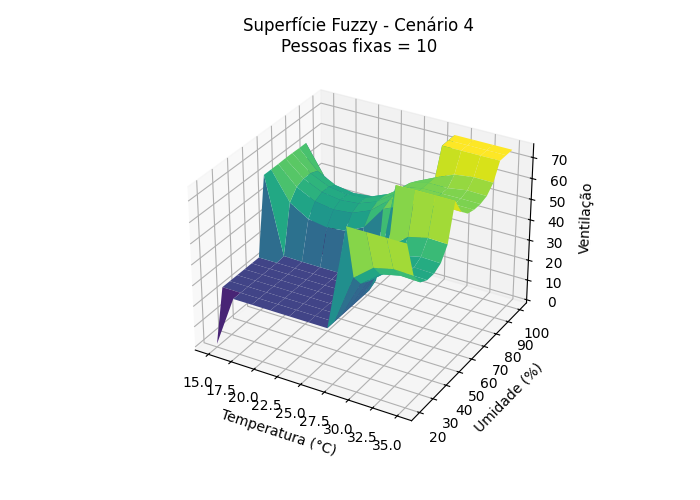
\includegraphics[width=0.48\textwidth]{../img/superficie_cenario4_fixapessoas.png}
    \caption{Ventilação em função de temperatura e umidade, pessoas fixas (Cenário 4).}
    \label{fig:superficie-c4-t-u}
\end{figure}
\begin{figure}[ht]
    \centering
    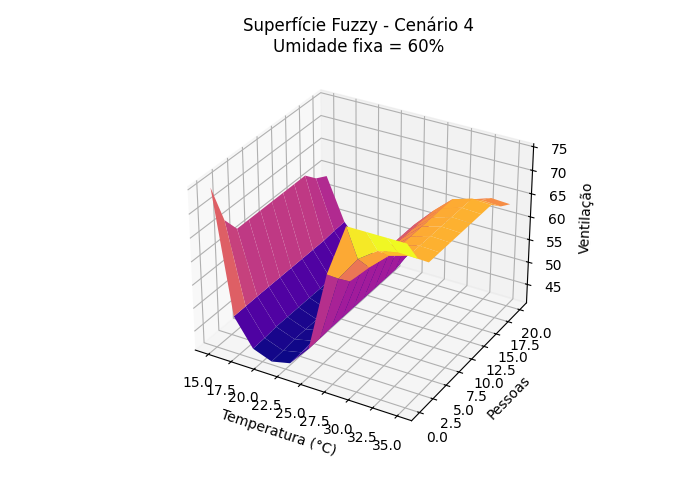
\includegraphics[width=0.48\textwidth]{../img/superficie_cenario4_fixaumidade.png}
    \caption{Ventilação em função de temperatura e pessoas, umidade fixa (Cenário 4).}
    \label{fig:superficie-c4-t-p}
\end{figure}
\begin{figure}[ht]
    \centering
    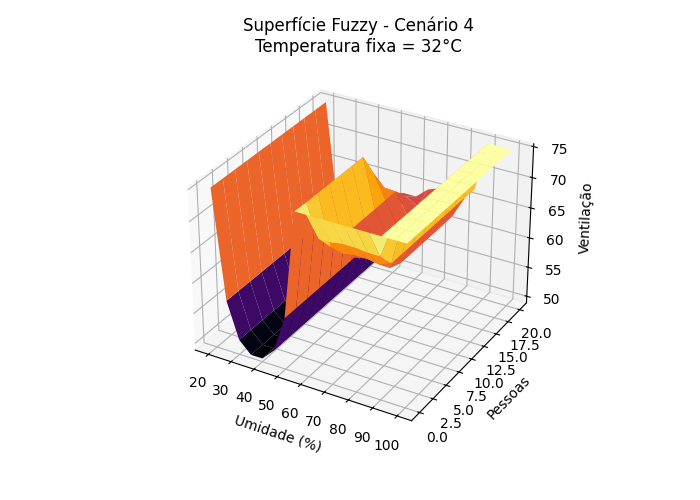
\includegraphics[width=0.48\textwidth]{../img/superficie_cenario4_fixatemperatura.png}
    \caption{Ventilação em função de umidade e pessoas, temperatura fixa (Cenário 4).}
    \label{fig:superficie-c4-u-p}
\end{figure}

Neste cenário, a ventilação recomendada é alta para temperaturas elevadas, mesmo com ocupação moderada, mostrando a influência dominante da temperatura.

\subsubsection{Cenário 5: Ambiente úmido e moderadamente ocupado}

As Figuras~\ref{fig:superficie-c5-t-u}, \ref{fig:superficie-c5-t-p} e \ref{fig:superficie-c5-u-p} apresentam as superfícies fuzzy para o Cenário 5.

\begin{figure}[ht]
    \centering
    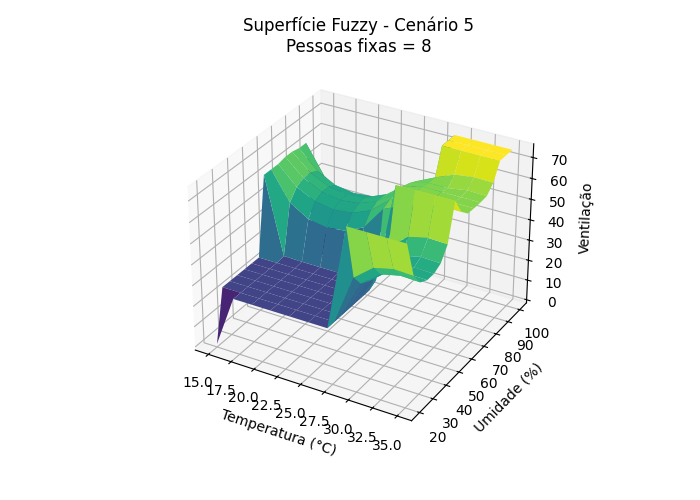
\includegraphics[width=0.48\textwidth]{../img/superficie_cenario5_fixapessoas.png}
    \caption{Ventilação em função de temperatura e umidade, pessoas fixas (Cenário 5).}
    \label{fig:superficie-c5-t-u}
\end{figure}
\begin{figure}[ht]
    \centering
    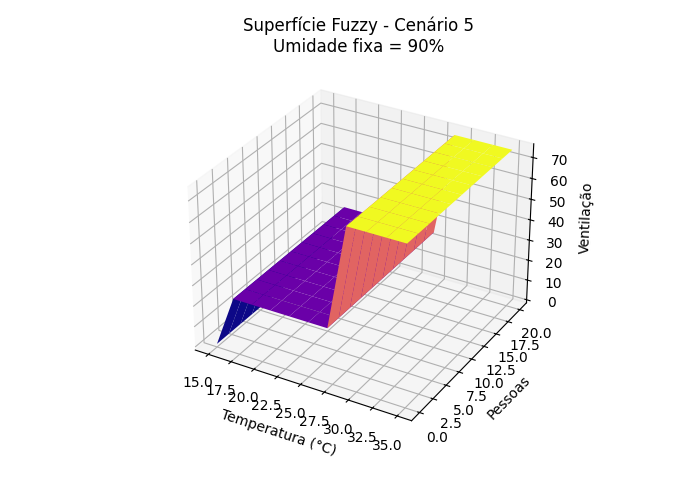
\includegraphics[width=0.48\textwidth]{../img/superficie_cenario5_fixaumidade.png}
    \caption{Ventilação em função de temperatura e pessoas, umidade fixa (Cenário 5).}
    \label{fig:superficie-c5-t-p}
\end{figure}
\begin{figure}[ht]
    \centering
    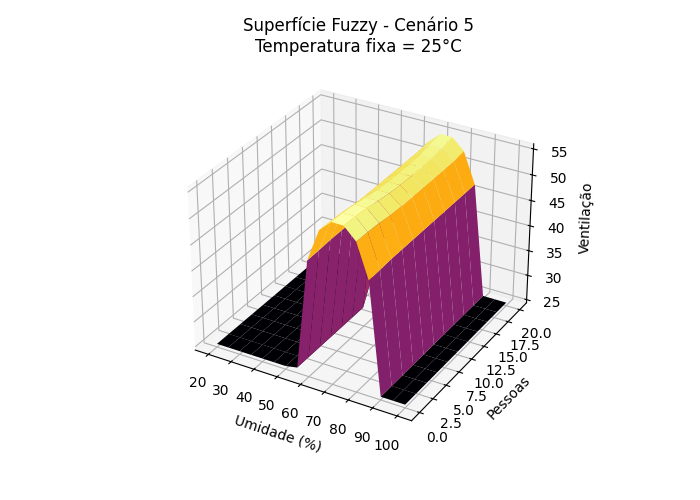
\includegraphics[width=0.48\textwidth]{../img/superficie_cenario5_fixatemperatura.png}
    \caption{Ventilação em função de umidade e pessoas, temperatura fixa (Cenário 5).}
    \label{fig:superficie-c5-u-p}
\end{figure}

No Cenário 5, a ventilação recomendada aumenta principalmente com o crescimento da umidade e do número de pessoas, mesmo para temperaturas intermediárias, evidenciando a importância da umidade no controle da ventilação.

\bigskip

Para cada cenário, o sistema fuzzy Mamdani realizou as seguintes etapas:

\begin{enumerate}
    \item \textbf{Fuzzificação:} Os valores de entrada (temperatura, umidade e número de pessoas) foram convertidos em graus de pertinência para os conjuntos fuzzy definidos.
    \item \textbf{Ativação das Regras:} Com base nesses graus, as regras fuzzy foram avaliadas e ativadas conforme o nível de firing strength.
    \item \textbf{Agregação da Saída Fuzzy:} As saídas das regras ativadas foram agregadas, formando uma função de pertinência fuzzy para a ventilação.
    \item \textbf{Defuzzificação:} Foram aplicadas as técnicas de centroide, média do máximo e bissetriz para obter o valor crisp da ventilação recomendada.
    \item \textbf{Visualização:} Para cada cenário, foi gerado um gráfico mostrando as funções de pertinência da saída, a área agregada e as linhas dos valores defuzzificados (Figuras~\ref{fig:defuzz-cenario1} a~\ref{fig:defuzz-cenario5}).
\end{enumerate}

A Tabela~\ref{tab:cenarios-regras-defuzz} apresenta de forma sintética os resultados dos cinco cenários simulados, incluindo os valores das entradas, as regras ativadas (com seus respectivos níveis de firing strength), o valor defuzzificado pelo método do centroide e a classificação qualitativa da ventilação recomendada. Dessa forma, o texto fica mais objetivo e a análise comparativa entre os cenários é facilitada.

\begin{table*}[ht]
\centering
\caption{Resumo dos cenários: entradas, regras ativadas e valor defuzzificado (centroide).}
\label{tab:cenarios-regras-defuzz}
\begin{tabular}{c|c|c|c|c|l|c}
\hline
\textbf{Cenário} & \textbf{Temperatura} & \textbf{Umidade} & \textbf{Pessoas} & \textbf{Centroide} & \textbf{Regras Ativadas} & \textbf{Intensidade} \\
\hline
1 & 28 & 80 & 15 & 62,44 & R1 (0,567), R6 (0,567), R9 (0,567) & Forte \\
2 & 22 & 50 & 5  & 24,98 & R3 (0,283), R7 (0,876)             & Fraca \\
3 & 18 & 30 & 2  & 24,98 & R3 (0,160), R7 (0,572)             & Fraca \\
4 & 32 & 60 & 10 & 66,88 & R1 (0,731), R6 (0,289), R9 (0,269) & Forte \\
5 & 25 & 90 & 8  & 24,98 & R7 (0,394)                         & Fraca \\
\hline
\end{tabular}
\end{table*}

A Figura~\ref{fig:defuzz-cenario1} a Figura~\ref{fig:defuzz-cenario5} ilustram, para cada cenário, a saída fuzzy agregada e os valores defuzzificados obtidos pelo método do centroide. Essas imagens permitem visualizar como a área agregada das funções de pertinência resulta no valor crisp final recomendado pelo sistema.

\begin{figure}[ht]
    \centering
    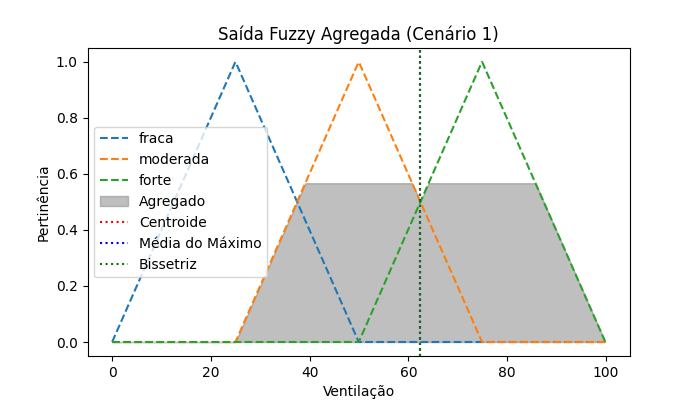
\includegraphics[width=0.45\textwidth]{../img/defuzz_cenario1.png}
    \caption{Saída fuzzy agregada e valor defuzzificado para o Cenário 1.}
    \label{fig:defuzz-cenario1}
\end{figure}

\begin{figure}[ht]
    \centering
    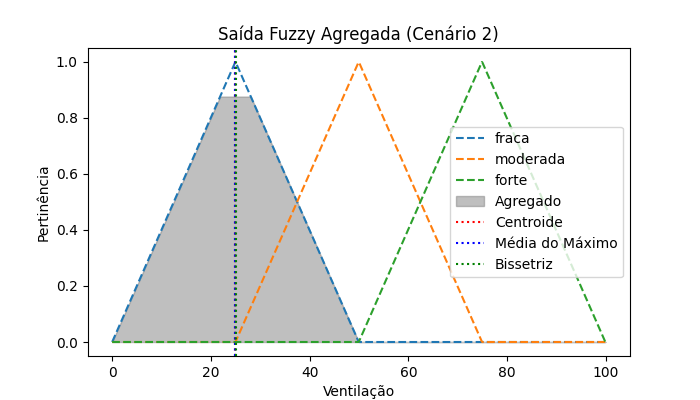
\includegraphics[width=0.45\textwidth]{../img/defuzz_cenario2.png}
    \caption{Saída fuzzy agregada e valor defuzzificado para o Cenário 2.}
    \label{fig:defuzz-cenario2}
\end{figure}

\begin{figure}[ht]
    \centering
    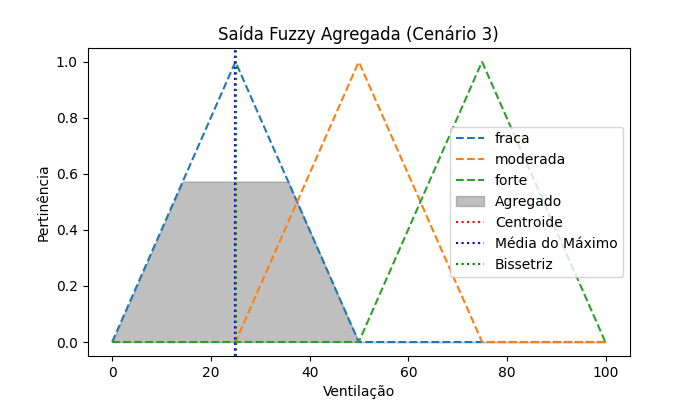
\includegraphics[width=0.45\textwidth]{../img/defuzz_cenario3.png}
    \caption{Saída fuzzy agregada e valor defuzzificado para o Cenário 3.}
    \label{fig:defuzz-cenario3}
\end{figure}

\begin{figure}[ht]
    \centering
    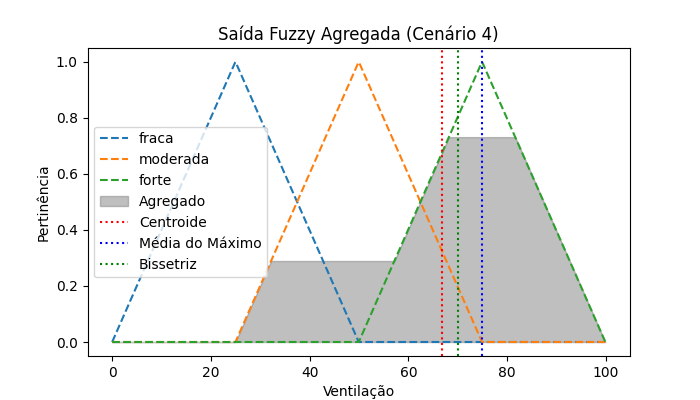
\includegraphics[width=0.45\textwidth]{../img/defuzz_cenario4.png}
    \caption{Saída fuzzy agregada e valor defuzzificado para o Cenário 4.}
    \label{fig:defuzz-cenario4}
\end{figure}

\begin{figure}[ht]
    \centering
    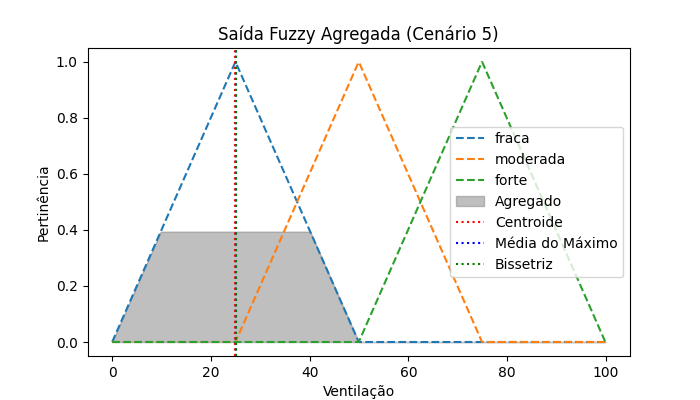
\includegraphics[width=0.45\textwidth]{../img/defuzz_cenario5.png}
    \caption{Saída fuzzy agregada e valor defuzzificado para o Cenário 5.}
    \label{fig:defuzz-cenario5}
\end{figure}

A análise dos dados da Tabela~\ref{tab:cenarios-regras-defuzz} e das Figuras~\ref{fig:defuzz-cenario1} a~\ref{fig:defuzz-cenario5} evidencia que o sistema fuzzy responde adequadamente às diferentes condições ambientais, recomendando ventilação mais intensa para cenários com altas temperaturas, umidade elevada ou maior número de pessoas, e ventilação fraca para ambientes amenos ou pouco ocupados. A classificação qualitativa facilita a comunicação dos resultados, permitindo ao usuário final compreender rapidamente a recomendação do sistema para cada situação. Mesmo com pequenas variações nos valores numéricos, a tendência qualitativa é robusta e condizente com o contexto de conforto térmico e eficiência energética.



